\documentclass[twocolumn]{article}
\usepackage{upquote}
\usepackage{listings}
\usepackage{color}
\usepackage[margin=1cm]{geometry}
 \usepackage{graphicx}
%\usepackage{wrapfig}
\begin{document}

\title{Autonomous Trading Agent Implementation Using Natural Language Processing Of News Headlines}
\author{William Lyon}
\date{\today}
\maketitle

\abstract{Natural Language Processing techniques are used to examine financial news headlines and generate predictions of stock price movements.  News headlines from the Wall Street Journal from January 1, 2009 to November 1, 2012 are collected and paired with daily S\&P 500 index returns.  This information is used to train a Naive Bayes classifier and generate BUY/SELL trading signals.  This trading strategy is then backtested using Wall Street Journal news headlines as a predictor for movement in the price of the S\&P 500 index. }

\section{Introduction}
In finance, the Efficient Market Hypothesis states that all publicly available information is reflected in financial market prices.  As new information becomes available, prices adjust to take this new information into account.  
\subsection{Motivation}
This tool could be used as a component of an autonomous trading agent that will make BUY/SELL decisions for trading financial instruments.
\subsection{Literature Review}

\section{Data}
Google Finance provides access to historical stock quotes as well as links to financial news stories pertaining to specific stocks. This data provides the basis for this paper.
\begin{figure}[htb]
%\begin{wrapfigure}{o}{8cm}
\centering
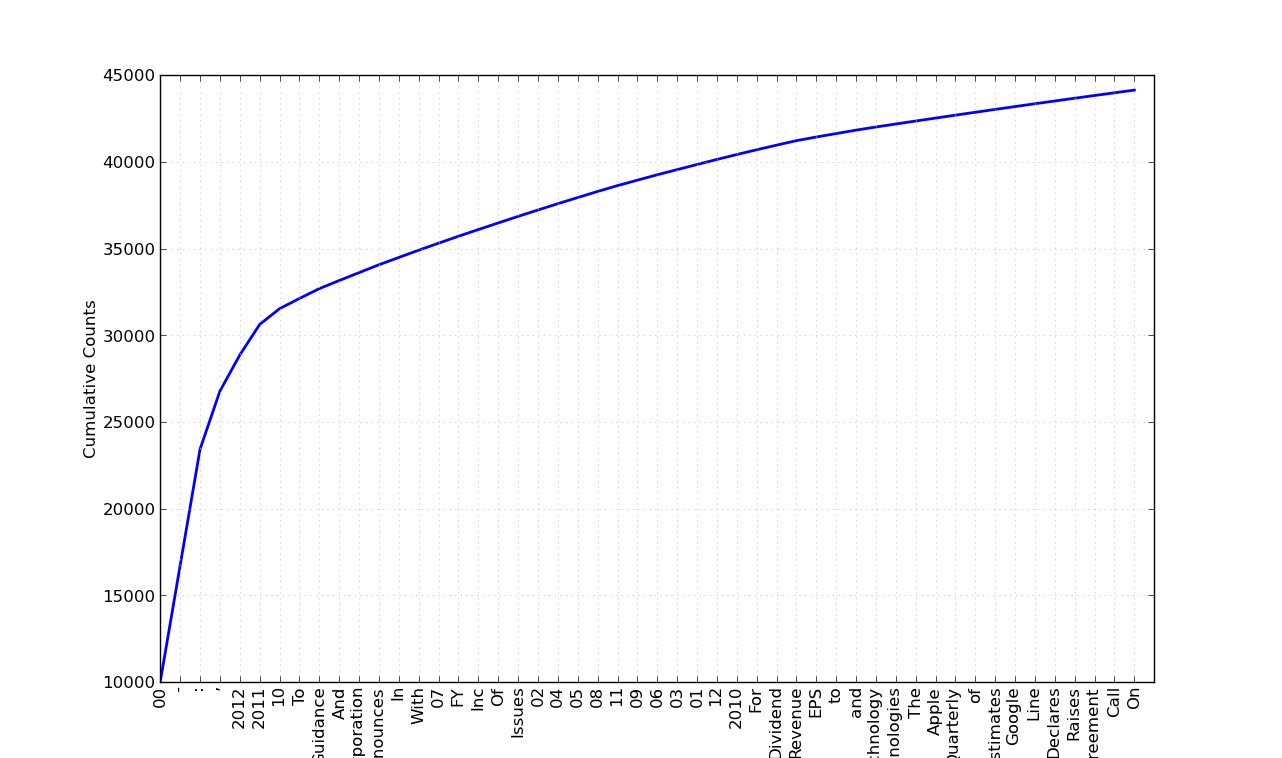
\includegraphics[scale=0.25]{cum_graph.png}
\caption{Cumulative frequency plot}
\end{figure}
%\end{wrapfigure}
%\end{figure}
%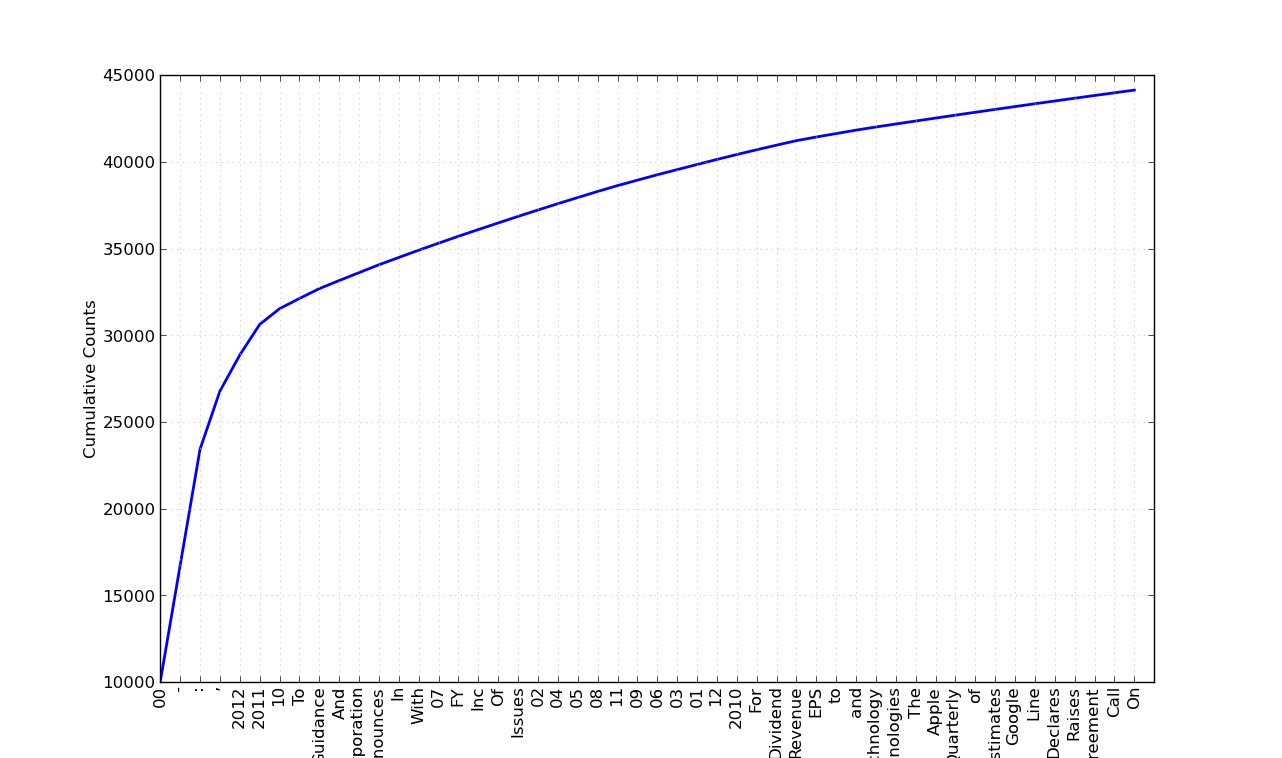
\includegraphics[width=60mm]{cum_graph.png}
%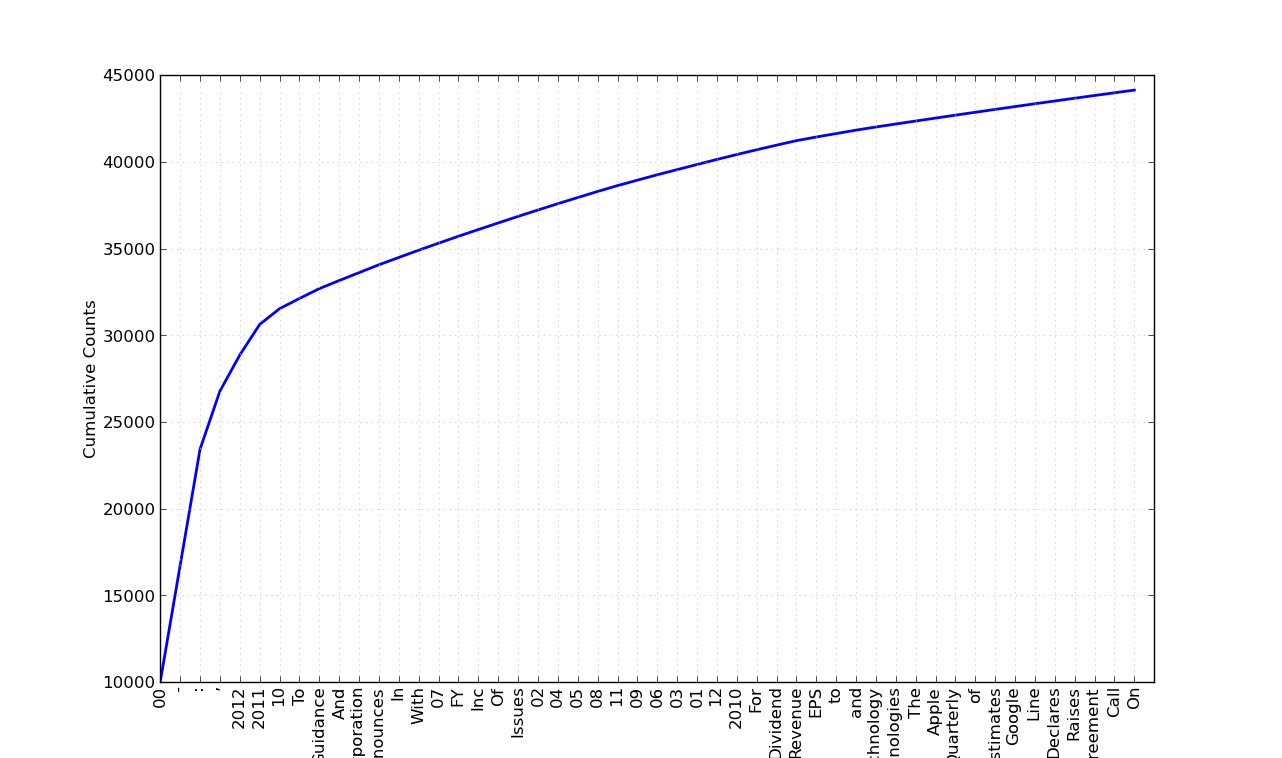
\includegraphics[height=60mm]{cum_graph.jpg}
%\includegraphics[scale=0.75]{myfig.pdf}
%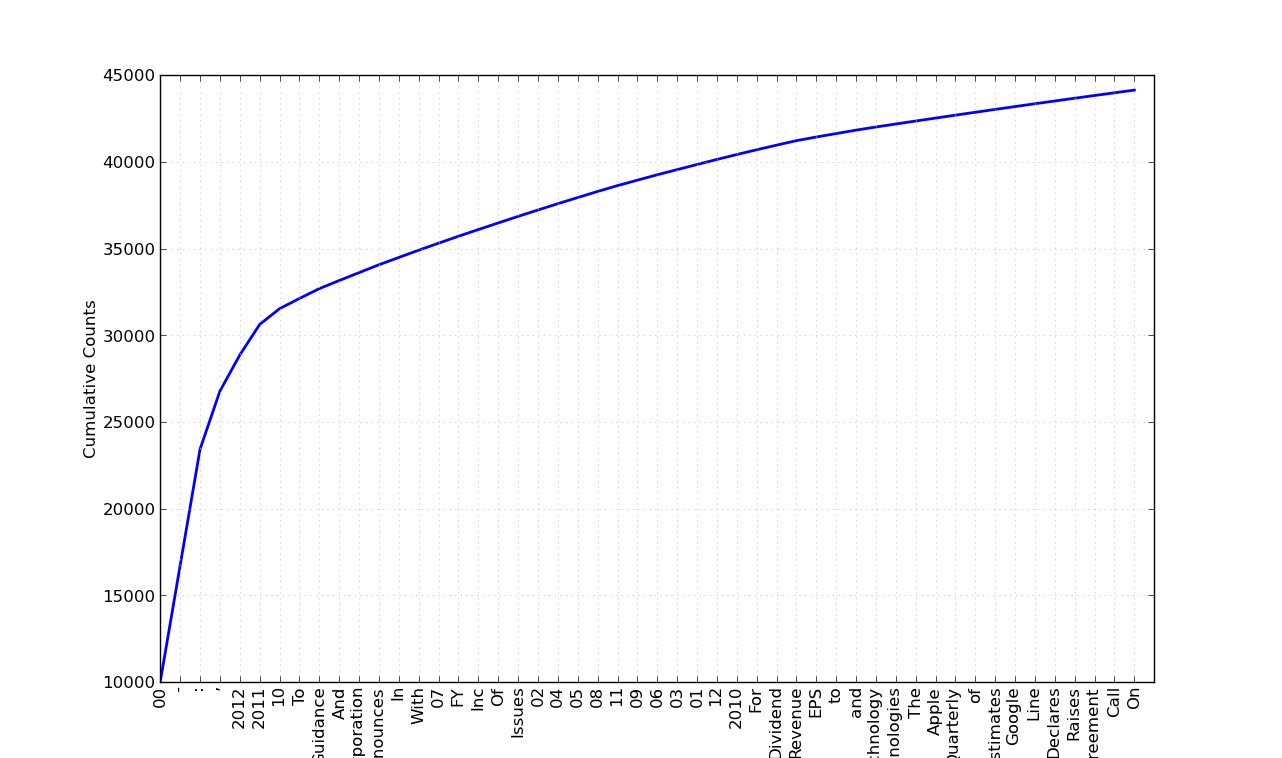
\includegraphics[angle=45,width=52mm]{cum_graph.png}
Here is some more text after the figure. The figure is somewhat floating i guess.  There is even more text after the figure.  

\section{Classification Methodology}
These tuples of [return, listOfDailyNews] are used as the training data for a Naive Bayes classifier. 
\subsection{Classes}

\subsection{Naive Bayes}


\section{Implementation}

\subsection{Dependencies}
\subsection{Data Collection \& Munging}
\subsection{Training NLP Classifier}
\subsection{Backtesting}
\section{Evaluation}
\subsection{Accuracy}

\subsection{Most informative features}

\subsection{Precision}

\subsection{Recall}

\section{Trading Model}
\subsection{Trading Signals}
\subsection{Backtesting}
\section{Conclusions}
\subsection{Further research}

\section{References}
\end{document}